\documentclass[letterpaper, 10 pt, conference]{ieeeconf}  

\IEEEoverridecommandlockouts
\overrideIEEEmargins

\usepackage{xparse} 
\usepackage{amsmath} 
\usepackage{amssymb}
\usepackage{amsfonts} 
\usepackage{bbm}
\usepackage{color}
\usepackage{resizegather}

\usepackage{graphicx}
\usepackage{epstopdf}
%\usepackage{caption}
%\usepackage{subcaption}

\usepackage{hyperref}
\usepackage{cleveref}
\usepackage{multirow}

% for biblatex and mklatex
\usepackage[backend=bibtex,style=ieee,natbib=true]{biblatex} %added
\addbibresource{ieeeabrv.bib} % Abbreviations
\addbibresource{main.bib} %added

\usepackage{nomencl} 
\makenomenclature

%mycal below
\graphicspath{{images/}}
\DeclareMathOperator*{\argmax}{\arg\max} %added by Mycal
\usepackage{adjustbox} %added by mycal
\usepackage{amsmath}
\usepackage{algorithm}
\usepackage[noend]{algpseudocode}

\title{DCG-UPUP-Away: Automatic Symbol Learning through Grounding to Unknowns}
\author{Mycal Tucker, Derya Aksaray, Rohan Paul, and Nicholas Roy% <-this % stops a space
\thanks{All authors are with the Computer Science and Artificial Intelligence Laboratory (CSAIL),
Massachusetts Institute of Technology, Cambridge, MA 02139, USA
{\tt\small \{mycal,daksaray,rohanp,nickroy\}@csail.mit.edu}}%
\thanks{It appears as if acknowledgments sometimes go here, but there's also the acknowledgment section at the end. What's the difference?}% <-this % stops a space
}

\begin{document}
\maketitle
\thispagestyle{empty}
\pagestyle{empty}

\begin{abstract}
This work addresses the symbol grounding problem, that is, understanding the ``meaning" of natural language within a robot's workspace. The state of the art models used in the grounding problem typically assume a fixed set of phrases or objects that are defined a priori to mission. However, the real world is full of unexpected objects that are nearly impossible to anticipate and therefore train for. This paper proposes a model called the ``Distributed Correspondence Graph - Unknown Phrase, Unknown Percept - Away" that explicitly represents unknown phrases and objects as unknown symbols and enables to reason about objects outside the field of view. Moreover, the model is capable of acquiring new symbols in an online fashion. The effectiveness of the model is evaluated via simulations and real experiments in terms of grounding and learning new phrases and objects.

%Research in automatic natural language grounding, the problem of robots associating phrases with realworld objects and actions, offers a tantalizing reality in which untrained humans can operate sophisticated robots. 

%Current techniques for training robots to understand natural language, however, assume that there is a fixed set of phrases or objects that the robot will encounter during deployment. 

%Instead, the real world is full of confusing jargon and unique objects that are nearly impossible to anticipate and therefore train for. 
%This paper presents a model called the Distributed Correspondence Graph - Unknown Phrase, Unknown Percept - Away (DCGUPUP- Away) that augments a previously successful model by explicitly representing unknown phrases and objects as unknown, as well as reasoning about objects that are not currently perceived. 
%Furthermore, experimental results in simulation,
%as well as a trial run on a physical turtlebot, validate the
%effectiveness of DCG-UPUP-Away in grounding and learning
%new phrases.
\end{abstract}

%\printnomenclature %I have no idea what this does

\section{Introduction}
Recently, there has been a great interest in human-robot teaming in civilian (e.g., at factories, hotels, hospitals, homes) and military (e.g., reconnaissance) applications. Communication plays an important role in effective teaming between humans and robots. One way of communication is via natural language, which provides a rich, intuitive, and flexible medium. Accordingly, the grounding problem in the literature addresses the question of how a robot can understand the meaning of a natural language command in the context of its world model (e.g., \cite{g3,dcg,adcg2016}). 
%However, this requires a robot to understand natural language commands  domains including, but not limited to, Robots must be able to understand natural language if they are to efficiently collaborate with humans. In order to achieve this goal, the problem of associating phrase with real-world objects and actions, commonly referred to as the grounding problem, has emerged as a focus of new research in robotics (\textcolor{blue}{REF: G3,DCG, etc.}).

The existing methods to solve the grounding problem make two primary assumptions. First, they assume a fixed set of phrases that can constitute the commands and a fixed set of objects that exist in the world model. Thus, such methods typically fail to reason about unknown phrases or objects that have never been encountered (e.g., in the training process).
Second, these methods often assume that the location of the object being grounded to is known (e.g., the phrases refer to the objects that are currently perceived or localized within a known map).
As a result, a robot using these methods tends to pick the most likely perceived grounding rather than exploring its surroundings.

Note that such assumptions do not typically reflect the reality. For example, humans tend to use context-specific lexicons in their daily life, or they often refer to objects whose locations may be unknown. To deal with such cases, training a robot to know the meaning of every possible word is infeasible and inefficient. Also, attempting to reason over the space of all possible maps is similarly computationally infeasible.

\begin{figure}[t]
	\centering
	\includegraphics[width=6cm]{intro_pic}
    \vskip-2ex	
	\caption{An illustration of the proposed model DCG-UPUP-Away, which has been trained only with cubes, spheres, and cylinders; and it may ground phrases to known perceived objects (1), unknown perceived objects (2), known hypothetical objects (3), or unknown hypothetical objects (4). [CHANGE FIGURE]}
	\vskip-1ex
	\label{fig:intro_pic}
\end{figure}
%To assume that language will be drawn from a fixed set and to assume that language only refers to known, perceived objects is unsafe in the real world.
%Humans regularly draw upon context-specific lexicons that the general population does not recognize; however, training a robot to know every possible meaning of every possible word is infeasible and inefficient.
%At the same time, humans often refer to objects whose locations are fundamentally unknown.
%Attempting to reason over the space of all possible maps, however, is similarly computationally infeasible.

This paper introduces a model called the Distributed Correspondence Graph - Unknown Phrase, Unknown Percept - Away (DCG-UPUP-Away), which relaxes two assumptions by 1) explicitly modeling unknown phrases and percepts, and 2) creating hypothetical objects outside the field of view.
These two changes yield a model that can ground a large variety of phrases in complex environments, and they facilitate learning new words and objects in an online fashion.
The proposed ideas are supported by a simulation study using commands generated by Amazon Mechanical Turk users.
Also, the performance of the model is evaluated via real experiments where a turtlebot is initially trained to recognize a small set of phrases and objects. The results demonstrate that the robot correctly grounds commands approximately 80\% of the time while learning new concepts in an unsupervised manner.

The remainder of this paper is organized as follows:
The preliminaries on probabilistic graphical models used for the grounding problem is introduced in Section~\ref{sec:background}.
The technical approach used in developing the DCG-UPUP-Away model is presented in Section~\ref{sec:technical}, and its implementation is presented in Section~\ref{sec:implementation}.
The model is evaluated in Section~\ref{sec:evaluation}.
Existing research in natural language robotics and human-robot interaction that complements this work are reviewed in Section~\ref{sec:related}. Finally, Sections~\ref{sec:conclusion} concludes the paper by summarizing the contributions and future research.

\section{Grounding Natural Language Instructions}
\label{sec:background}
The work in this paper falls within the field of natural language grounding, which addresses the problem of correctly determining how phrases relate to the real world (e.g., the phrase ``go to the cube'' means approaching a physical cube).
% Before proceeding further, one must define the domains over which the grounding problem may be solved.
To this end, the general grounding problem can be formulated as a probability maximization problem
\begin{equation}
\boldsymbol{\gamma}^* = \argmax_{\boldsymbol{\gamma} \in \Gamma^{|\boldsymbol{\lambda}|}} p(\boldsymbol{\gamma}|\boldsymbol{\lambda},\Upsilon),
\label{eq:max_ground_prob}
\end{equation}
where $\boldsymbol{\lambda}$ is the natural language command that is a vector of phrases from the set $\Lambda$ (i.e.,  the set ${\Lambda = \{\text{English phrases}\}}$ represents what phrases natural language sentences may be composed of); $|\boldsymbol{\lambda}|$ is the length of the natural language command; ${\Gamma}$ is the set of groundings that correspond to semantic notions such as objects, locations, regions, paths, or actions the robot can take and $\boldsymbol{\gamma} \in \Gamma^{|\boldsymbol{\lambda}|}$ is a vector of groundings with a length of $|\boldsymbol{\lambda}|$; and $\Upsilon$ denotes the physical workspace of the robot that aggregates metric and semantic information about the constituent objects. In this formulation, the optimal vector of groundings $\boldsymbol{\gamma}^*$ is the one with maximum likelihood, given a command $\boldsymbol{\lambda}$ and a world model $\Upsilon$.

%the cartesian product of the set of objects (i.e., $\boldsymbol{\Gamma^O} \subset \boldsymbol\Gamma$) and the object attributes (e.g., color, location), which represents the world model in which the phrases may be grounded. 

%In the general formulation of the grounding problem, three sets must be considered: ${\Gamma = \{\text{symbolic actions and objects\}}}$ is the set of groundings, which represents what phrases may be grounded to; ${\Lambda = \{\text{English phrases}\}}$ is the set of phrases, which represents what phrases natural language sentences may be composed of; and ${\Upsilon = \Gamma^O \times \{\text{object attributes}\} }$ is the cartesian product of the set of objects (i.e., $\Gamma^O \subset \Gamma$) and the object attributes (e.g., color, location), which represents the world model in which the phrases may be grounded. 

%Given a natural language command $\boldsymbol{\lambda}$, which is a vector of phrases from the set $\Lambda$ and has a length of $|\boldsymbol{\lambda}|$, 
%%\indent Using these domains, it is possible to formulate 
%the general grounding problem can be formulated as a probability maximization problem%, shown in Equation~\ref{eq:max_ground_prob},
%\begin{equation}
%\boldsymbol{\gamma}^* = \argmax_{\boldsymbol{\gamma} \in \Gamma^{|\boldsymbol{\lambda}|}} p(\boldsymbol{\gamma}|\boldsymbol{\lambda},\Upsilon),
%\label{eq:max_ground_prob}
%\end{equation}
%where $\boldsymbol{\gamma} \in \Gamma^{|\boldsymbol{\lambda}|}$ is a vector of groundings with a length of $|\boldsymbol{\lambda}|$, and $\Upsilon$ denotes the world model. 
%$\gamma \in \Gamma$, $\boldsymbol{\lambda}$ as a vector of phrases $\lambda \in \Lambda$ and world model $\Upsilon$. 


In practice, the domains of $\Gamma$, $\Lambda$, and $\Upsilon$ in \eqref{eq:max_ground_prob} typically include elements from previously seen examples. % While the general formulation allows any possible grounding, phrase, or world model, the domains of $\Gamma$, $\Lambda$, and $\Upsilon$ are shrunk in existing solutions to the grounding problem.
For example, rather than allowing the set of phrases $\Lambda$ to include all words in a dictionary, $\Lambda$ is generally assumed to only contain words that have appeared in the training examples. Moreover, solving \eqref{eq:max_ground_prob} is a hard combinatorial optimization problem due to the diversity in language and world.
% even though limited sets ($\Gamma$, $\Lambda$, and $\Upsilon$) are considered. 
%For example, the Generalized Grounding Graph (G3) model \cite{g3} is a factor graph that is trained from a corpus of labeled examples to ground language commands with objects, locations, and paths.  

One way to tackle the complexity of solving \eqref{eq:max_ground_prob} is modeling it as an inference over a probabilistic graphical model based on the linguistic structure of the commands. In literature, there exists an efficient model called the Distributed Correspondence Graph (DCG) \cite{dcg}, which discretizes the continuous space of groundings ($\Gamma$) as regions and motion constraints and introduces correspondence variables ($\phi_{ij}$) relating the $i^{th}$ phrase $\lambda_i$ with the $j^{th}$ grounding variable $\gamma_{ij}$. The DCG model mainly assumes the grounding variables as conditionally independent and solves an inference problem as a search over the unknown correspondence variables as follows: 
\begin{equation}
\label{eq:dcg_factored1}
\begin{split}
\boldsymbol{\phi}^* = \argmax_{\phi_{ij} \in \boldsymbol{\phi}} \prod_{i}^{| \boldsymbol{\lambda}|} \prod_{j}^{|\Gamma_i|} p(\phi_{ij}|\gamma_{ij},\lambda_i, \Phi_{c_{i}}, \Upsilon_{KP}),
\end{split}
\end{equation}
where $\lambda_i \in \Lambda_{KN}$ and $\Lambda_{KN}$ is the set of phrases with known (previously seen) words; $\Gamma_i$ is the set of grounding variables of $\lambda_i$ \footnote{If $\lambda_i$ is a noun phrase, the corresponding grounding set $\Gamma_i$ contains the objects in the world (i.e., $\Gamma^O$). If $\lambda_i$ is a verb phrase referring to the actions that the robot can take (e.g., ``move", ``pick"), then $\Gamma_i$ contains the regions discretized with respect to the objects under consideration (i.e., $\Gamma^{RO}$).}, $\phi_{ij}$ is the $j^{th}$ correspondence variable of $\lambda_i$; $\gamma_{ij}$ is the $j^{th}$ grounding of $\lambda_i$; $\Upsilon_{KP}$ denotes the world model consisting of the set of known perceived symbolic objects and regions; and  $\Phi_{c_{i}}$ is the set of child correspondence variables of $\lambda_{i}$. Note that $\Phi_{c_{i}}$ is defined as the set of correspondance variables for the immediate children phrases (leftmost descendants) of the parent phrase $\lambda_i$ in the parse tree of the natural language command. Accordingly, the DCG infers the most likely set of planning constraints from the language commands.

For example, consider Fig.~\ref{fig:parse_tree} that shows the parse tree of a simple command (\emph{``move to the cube"}), and Fig.~\ref{fig:dcg_plates} that shows the corresponding DCG model. The child correspondence variable of the phrase ``move'' is the correspondence variable for the phrase ``to.'' Similarly, the child correspondence variable of the phrase ``to'' is the correspondence variable for the phrase ``the cube'' \footnote{The determiners such as ``the'' may be collapsed into their nouns}. Thus, in this example, each correspondence variable has exactly one child correspondence variable, yielding the inter-plate structure in Fig.~\ref{fig:dcg_plates}.
Examining the parse tree also reveals why the factorization in \eqref{eq:dcg_factored1} is reasonable: the meaning ``move'' should be conditionally independent of the noun ``cube'' given the prepositional phrase.
After all, the correct grounding of the word ``move'' is an action that does not depend on whether the target is a cube or a sphere, but it does depend on the position of the cube.

  %(rather than grounding phrases to particular actions, objects, or paths as in G3 model). 
%In particular, the DCG model has the following properties:  
%First, the DCG decouples motion planning from the grounding problem. To this end, it discards the notion of grounding to specific actions or objects by instead only grounding to constraints relative to known objects (e.g. the area near a cube). Then, it passes the constraints to a motion planner.
%Second, the DCG allows only the phrases composed entirely of the words that have already been encountered in training.
%Third, the DCG only considers the perceived objects rather than a full model of the world including the unobserved objects.
%Fourth, ternary correspondence variables $\phi_{ij}$ are introduced to represent whether the $i^\text{th}$ phrase $\lambda_i$ from the overall command $\boldsymbol{\lambda}$ corresponds to a grounding $\gamma_{ij}$.
%For a given phrase $\lambda_i$, $\phi_{ij}$ is set to \emph{Active} if $\lambda_i$ refers to constraint $\gamma_{ij}$ (e.g., the area near the cube), \emph{Inverted} if $\lambda_i$ refers to the opposite of $\gamma_{ij}$ (e.g. the area far from the cube), or \emph{Inactive} if $\lambda_i$ has no bearing on $\gamma_{ij}$ (e.g. the area near a sphere).
%Fifth, for the sake of computational efficiency, the overall inference is factored using conditional independence according to the structure of the parse tree of $\boldsymbol{\lambda}$.

%Accordingly, the optimization problem solved over a DCG model becomes
%\begin{equation}
%\label{eq:dcg_factored1}
%\begin{split}
%\boldsymbol{\phi}^* = \argmax_{\phi_{ij} \in \boldsymbol{\phi}} \prod_{i}^{|\boldsymbol{\lambda}|} \prod_{j}^{|\Phi_i|} p(\phi_{ij}|\gamma_{ij},\lambda_i,\Gamma_{c_{ij}} , \Upsilon_{KP}),
%\end{split}
%\end{equation}

%Finally, the domains are redefined for $\gamma \in C=\{\text{Constraints}\}$, $\lambda \in \Lambda_{KN}=\{\text{phrases with known nouns}\}$, and $\Upsilon \in \{\text{object attributes}\} \times \Gamma_{KP}$ for $\Gamma_{KP} = \{\text{known perceived symbolic objects}\}$.\\
%\indent As stated previously, DCG assumes conditional independence among groundings, given $\Gamma_{c_{ij}}$.
%Child groundings $\Gamma_{c_i}$ may be formally defined as the set of groundings for the leftmost descendants of the immediate children (barring itself) of the parent of phrase $i$ in the parse tree of the natural language command.


\begin{figure}[h!]
\centering
\begin{subfigure}[b]{0.38\columnwidth}
\includegraphics[width=\textwidth]{parse_tree}
\caption{Parse tree for the command ``move to the cube''}
\label{fig:parse_tree}
\end{subfigure}
~
\begin{subfigure}[b]{0.58\columnwidth}
\centering
\includegraphics[width=\textwidth]{dcg_plates_new.pdf}
\caption{The DCG graphical model for the parse tree in Fig.~\ref{fig:parse_tree}}
\label{fig:dcg_plates}
\end{subfigure}
\caption{An illustration of a parse tree and the corresponding DCG model.}
\end{figure}

Finally, the equation in \eqref{eq:dcg_factored1} can be factorized as \eqref{eq:llm1}, where the factor function $\Psi : \Phi \times \Gamma \times \Lambda \times \Phi \times \Upsilon \rightarrow
 \mathbb{R}$ (e.g., within each plate in Fig.~\ref{fig:dcg_plates}) determines the most likely configuration $\boldsymbol{\phi^*}=\{\phi_{11}, \phi_{12}, \dots\}$ (where each $\phi_{ij} \in \Phi$) given $\gamma_{ij} \in \Gamma_i$, $\lambda_i \in \boldsymbol\lambda$, $\Phi_{c_{i}} \subset \Phi$, and $\Upsilon_{KP} \subset \Upsilon$. %Accordingly, one may rewrite \eqref{eq:dcg_factored1} as
%In order to expose the use of $\Psi$, one may rewrite Equation~\ref{eq:dcg_factored1} as Equation~\ref{eq:llm1}, \\
\begin{equation}
\boldsymbol{\phi}^* = \argmax_{\phi_{ij} \in \Phi} \prod_{i}^{\boldsymbol{|\lambda|}} \prod_{j}^{|\Gamma_i|} \Psi(\phi_{ij},\gamma_{ij},\lambda_i,\Phi_{c_{i}},\Upsilon_{KP}).
\label{eq:llm1}
\end{equation}

\color{blue} 
EXPLAIN training - features
where $\Psi$ is a log-linear model composed of a weighted combination of hand-coded binary functions, that is,
\begin{equation}
\Psi(\phi_{ij},\gamma_{ij},\lambda_i,\Phi_{c_{i}},\Upsilon_{KP}) = \frac {\exp \Big( \sum\limits_{f \epsilon F} \mu_f f(\phi_{ij},\gamma_{ij},\lambda_i,\Phi_{c_{i}},\Upsilon_{KP}) \Big)}{\sum\limits_{\phi_{ij} \in \{-1,0,1\}}\exp \Big( \sum\limits_{f \epsilon F} \mu_f f(\phi_{ij},\gamma_{ij},\lambda_i,\Phi_{c_{i}},\Upsilon_{KP}) \Big)},
\label{eq:llm2}
\end{equation}
where each binary function $f$ belongs to a set of hand-coded binary features that evaluate specific traits about a grounding (e.g., whether the word ``cube'' appears in $\boldsymbol{\lambda}$), and $\mu_f$ is the weighting of each $f$. In this work,
the weights $\mu_f$ are learned in a training procedure via the Limited-memory Broyden-Fletcher-Goldfarb-Shanno algorithm.% to generate a more nuanced function that evaluates how likely a phrase is to correspond to a grounding.
\color{black}

Note that a limitation of the DCG model is that it assumes a fixed set of symbols (i.e., objects and phrases) so it does not explicitly represent the unknown symbols. Thus, this model is unable to reason about objects and phrases that have not been trained on. 
\section{Technical Approach} \label{sec:technical}
technical dev goes here

I've written up the pseudo-code here so we can refer to it later:\\
\begin{algorithm}
\caption{My algorithm}\label{alg:dcg_upup_away}
\begin{algorithmic}[1]
\Procedure{DCG-UPUP-Away}{}
\State $M \gets \text{new DCG-UPUP-Away}$
\State $M.\Gamma \gets \text{init\_groundings}$
\State $M.F \gets \text{init\_features}$
\State $T \gets \text{init\_training}$
\State $M.\text{train}(M.\Gamma, M.F, T)$
\While {true}
\State $\Upsilon \gets \text{perceive\_objects}(\text{camera},M.\Gamma)$
\State $\Upsilon \gets \Upsilon + \text{hypothesize\_objects}(M.\Gamma)$
\State $\boldsymbol{\lambda} \gets \text{get\_nl\_command}()$
\State $[\boldsymbol{\phi}^*,\boldsymbol{\gamma}^*] \gets M.\text{ground}(\boldsymbol{\lambda},\Upsilon)$
\If {$\boldsymbol{\gamma}^*.\text{is\_hypothesized}()$}
\State $\text{spin\_in\_place()}$
\Else
\State $\text{drive\_to}(\boldsymbol{\gamma}^*)$
\EndIf
\State $T_u \gets \text{gen\_unsupervised\_training}(\boldsymbol{\lambda},\boldsymbol{\gamma}^*,\Upsilon)$
\If {$\text{is\_unknown}(\boldsymbol{\lambda}) \& !\boldsymbol{\gamma}^*.\text{is\_hypothesized}()$}
\State $\gamma' \gets \text{new\_grounding}(\boldsymbol{\lambda},\boldsymbol{\gamma}^*,\Upsilon)$
\State $M.\Gamma \gets M.\Gamma + \gamma'$
\State $M.F \gets M.F + f_{\text{word}}(\boldsymbol{\lambda}[\text{noun}])$
\State $M.F \gets M.F + f_{\text{obj}}(\boldsymbol{\gamma}^*[\text{obj}])$
\State $T_u \gets \text{replace\_unknown}(T_u,\gamma')$
\EndIf
\State $T \gets T + T_u$
\State $M.\text{train}(M.\Gamma, M.F, T)$
\EndWhile
\EndProcedure
\end{algorithmic}
\end{algorithm}
\section{Evaluation}
\label{sec:evaluation}
%\subsection{Experimental Setup}
The performance of the DCG-UPUP-Away model is demonstrated in two experiments.
First, a simulated TurtleBot within randomly generated simulated environments is given a series of user-generated natural language commands.
Second, an actual TurtleBot is given specific commands in a laboratory environment in order to demonstrate novel behaviors enabled by the DCG-UPUP-Away model.
Both experiments assume a perfect object recognizer that translates the raw sensor data into a world model, as well as an initial set of hand-labeled training examples for training the log-linear model to ground cubes, spheres, and cylinders.
In all trials, training the model with $55$ positive examples took less than $1$ minute on a Lenovo Thinkpad X1 Carbon, and grounding a command took under $40$ seconds.
%\subsection{Experimental Setup}

\subsection{Corpus}
The simulated testing environments are randomly generated in Gazebo.
Ten worlds are created, and each is populated with a random collection of objects in randomized locations.
In this work, we consider $8$ possible object types (including cubes, spheres, and cylinders) in $3$ possible colors (red, blue, green), for a total of $24$ objects.
Each object has a $15\%$ chance of being added to a given map.
Using such a procedure to generate environments coupled with the limited field of view of the TurtleBot has caused $87\%$ of the objects to be placed outside the initial field of view of the robot, which demonstrates the need for the ability to ground commands to hypothesized objects.

After generating the 10 worlds, the screen shots of a world with a highlighted single object are uploaded to Amazon Mechanical Turk. For each image, the users were instructed to write a command ``for approaching the highlighted object.''
These image-command pairs were saved for evaluating whether a robot, when placed in the corresponding simulated world and given the natural language command, successfully approaches the correct object.
An example screen shot, with an annotation supplied by a user, is shown in Fig.~\ref{fig:amt}.
\begin{figure}[htb!]
	\centering
    \includegraphics[width=7.5cm]{amt}
	\caption{A simulated world with a highlighted object presented on Amazon Mechanical Turk, labeled by a user as ``Move to the red fire hydrant.''}
	\label{fig:amt}
\end{figure}
\subsection{Testing/Training Setup}
Ten image-command pairs are randomly selected without any replacement from the pool of all pairs.
Note that a trial along the paper refers to $10$ ordered pairs, and each specific pair is called one iteration.
Accordingly, $30$ trials are generated, each consisting of $10$ iterations, for a total of $300$ evaluations.
When executing a trial, the TurtleBot is first trained on the initial, hand-curated training set.
The robot is then given the natural language command from the first iteration, and then retrained using the initial data supplemented by unsupervised training examples generated by the first iteration.
The retrained TurtleBot is given the command from the next iteration, and appropriately retrained after each execution until all 10 iterations have been executed.

\section{Results}
This section presents the performance results of the DCG-UPUP-Away model based on the grounding accuracy (how likely the model correctly grounds a phrase) and the number of known symbols.
Under the grounding accuracy results, we also examine when phrases are grounded to known, unknown, or learned objects.
\subsection{Grounding Accuracy}
%The primary metric used in evaluating the success of DCG-UPUP-Away is the grounding accuracy: how likely is the TurtleBot to correctly execute the natural language command.
As discussed previosuly, the TurtleBot is retrained between the iterations, thus the grounding accuracy may change as a function of iteration number. In fact, the mean grounding accuracy remains between $70\%$ and $90\%$ across all iterations, as shown in Figure~\ref{fig:g_acc}. Although the overall grounding accuracy remains relatively constant, the underlying behavior within the DCG-UPUP-Away model changes over the course of a trial. For example, Fig.~\ref{fig:g_acc_split} illustrates 3 curves showing what fraction of correctly grounded phrases refer to known, unknown, or learned objects as a function of iteration number. In the first iteration, nearly $70\%$ of correctly grounded commands refer to known objects, but by the 10$^\text{th}$ iteration that number has fallen to nearly $10\%$, replaced almost entirely by correctly grounding to learned objects.

\begin{figure}[htb!]
%\centering
%\begin{subfigure}[b]{0.9\columnwidth}
\centering
\includegraphics[width=0.75\columnwidth]{g_acc}
\caption{The overall grounding accuracy over various iterations.}
\label{fig:g_acc}
\end{figure}

\begin{figure}[htb!]
%\begin{subfigure}[b]{0.85\columnwidth}
\centering
\includegraphics[width=0.75\columnwidth]{symbols_corr}
\caption{The number of new symbols acquired during the simulations.}
\label{fig:symbols}
%\end{subfigure}
%\caption{The performance results of the simulation study.}
\end{figure}

\begin{figure}[htb!]
\centering
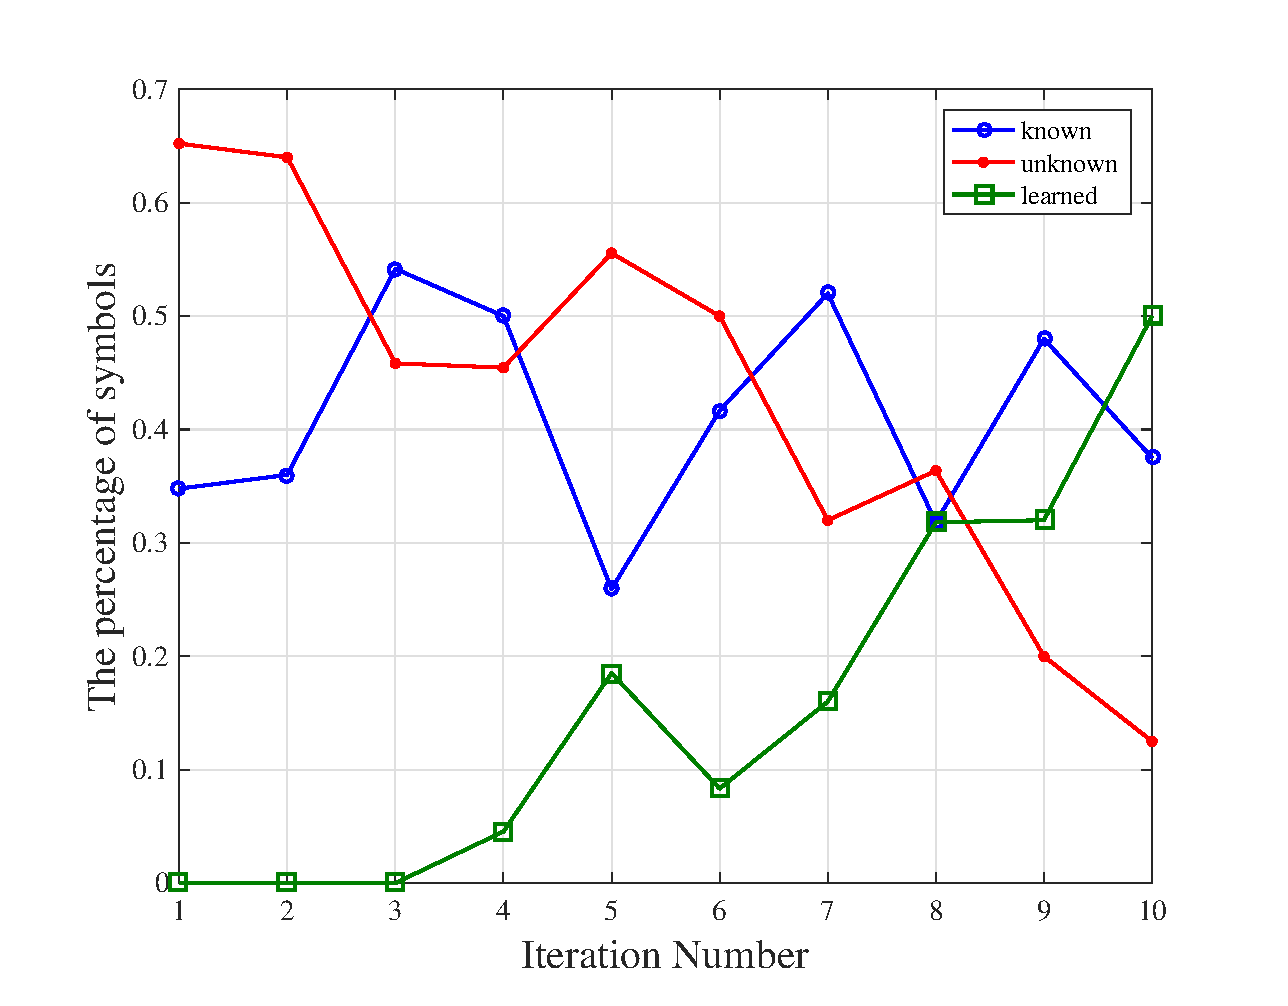
\includegraphics[width=0.8\columnwidth]{split_cases.eps}
\caption{The percentage of known, learned, and unknown symbols during the simulations.}
\label{fig:g_acc_split}
\end{figure}


%\begin{figure}[h]
%\centering
%\includegraphics[width=8.5cm]{learning}
%\caption{this is split up (must replot well)}
%\label{fig:g_acc_split}
%\end{figure}


\subsection{Learned Symbols}
In order to better examine the learning behavior exhibited by the DCG-UPUP-Away model, the other performance metric considered is the number of correctly known symbols. Note that the symbols may be incorrectly learned by associating a phrase with the wrong sort of object due to the nature of unsupervised learning.
Initially, the TurtleBot is trained with cubes, spheres, and cylinders, but the generated environments may contain up to 5 additional object types (i.e., fire hydrants, drills, mailboxes, door handles, and traffic cones).
Whenever an unknown phrase is grounded to such an unknown object, the TurtleBot learns the new symbol.
Thus, one may calculate the expected number of known symbols as a function of the iteration number using combinatorics to count how many unknown objects are present.
The recorded number of correctly learned symbols are plotted in Fig.~\ref{fig:symbols} in blue, as well as the expected number in red.
%\begin{figure}[h]
%\centering
%\includegraphics[width=8.5cm]{symbols_corr}
%\caption{this is how we show that we learn symbols. I will update this label (and caption) of this figure. also must use std error bars instead of variance}
%\label{fig:symbols}
%\end{figure}
%(Asking for advice: the x axis ranges from 1 to 11 because I can retrain after the 10th iteration and increase the mean number of symbols learned. It's a small increase, though, so I wouldn't be too upset cutting off the 11th iteration, though.)

As expected, the blue curve starts at $3$ (for the cube, sphere, and cylinder), and stochastically monotonically increases.
In $10\%$ of the trials, all $8$ symbols were correctly learned. In other trials the DCG-UPUP-Away model incorrectly grounded unknown phrases (and therefore learned an incorrect symbol) or the 10 iterations collectively never referred to the five initially unknown objects, preventing the DCG-UPUP-Away model from ever learning the new symbol.
Furthermore, learning symbols correctly improves the grounding accuracy: for each additional correctly learned symbol, the TurtleBot is over $4\%$ more likely to correctly ground a command. %(TODO generate p values via ANOVA.)

\subsection{Physical Demonstration}
\begin{figure*}[t!]
\begin{subfigure}[b]{0.155\textwidth}
\centering
\includegraphics[width=\textwidth]{1.png}
\caption{t=0 sec.}
\label{fig:exp1}
\end{subfigure}
~
\begin{subfigure}[b]{0.155\textwidth}
\centering
\includegraphics[width=\textwidth]{2.png}
\caption{t=25 sec.}
\label{fig:exp2}
\end{subfigure}
~
\begin{subfigure}[b]{0.155\textwidth}
\centering
\includegraphics[width=\textwidth]{3.png}
\caption{t=50 sec.}
\label{fig:exp3}
\end{subfigure}
~
\begin{subfigure}[b]{0.155\textwidth}
\centering
\includegraphics[width=\textwidth]{4.png}
\caption{t=70 sec.}
\label{fig:exp4}
\end{subfigure}
~
\begin{subfigure}[b]{0.155\textwidth}
\centering
\includegraphics[width=\textwidth]{5.png}
\caption{t=95 sec.}
\label{fig:exp5}
\end{subfigure}
~
\begin{subfigure}[b]{0.155\textwidth}
\centering
\includegraphics[width=\textwidth]{6.png}
\caption{t=120 sec. }
\label{fig:exp6}
\end{subfigure}
\caption{An illustration of grounding to a hypothetical object. The robot initially knows all objects in the world other than a crate. The TurtleBot is given a command as ``move towards the crate". (a) First, it does not see an unknown object in its perceived world so it creates a hypothetical unknown object, (b,c,d) it explores the world by rotating at its current location until it perceives an unknown object, (e) It perceives an unknown object and grounds to it, (f) it drives to the crate.}
\label{fig:crate}
\end{figure*}
In addition to the simulation studies, the DCG-UPUP-Away model was tested on an actual TurtleBot in a laboratory setting.
The TurtleBot was placed facing %a cylinder (known) and 
a cone (unknown).
In addition, a cube (known) and a crate (unknown) were located behind the TurtleBot.
All objects were labeled with the April tags \cite{olson2011}, which were used to generate the world model $\Upsilon$ from a kinect camera mounted on the TurtleBot.

%I'd like to add a footnote saying that I have videos of these demos
Three natural language commands were used to demonstrate various capabilities of the DCG-UPUP-Away model.
%First, the TurtleBot was given the command ``move towards the cube.''
%The TurtleBot successfully drove to the cube, demonstrating a correct grounding to a known, perceived object.\\
First, the TurtleBot was given the command ``move towards the cone.''
The TurtleBot drove to the cone, demonstrating that it perceived the cone as unknown, recognized the phrase ``cone'' as unknown, and grounded the unknown phrase to the unknown object.
Thus, a command was correctly grounded to an unknown perceived object as illustrated in Fig.~\ref{fig:cone}.
Second, the TurtleBot was given the command ``move towards the cube.''
The TurtleBot rotated in place until the cube came in perception, and then approached the cube.
In other words, the command was first grounded to a known hypothesized object, and then it was grounded to a known perceived object once the cube was seen. 
Finally, the TurtleBot was given the command ``move towards the crate.''
Once again, the TurtleBot explored its surrounding by rotating at its current location and drove to the crate once it perceived it (as illustrated in Fig.~\ref{fig:crate}). %rotated in place, this time until it saw the crate, whereupon it drove to the crate.

The experimental results demonstrate two important behaviors: 1) the TurtleBot must have learned what a cone was, otherwise the unknown phrase ``crate'' would have been grounded to the cone, and 2) the TurtleBot grounded the command to an unknown hypothesized object until the crate was perceived. The interested reader is referred to the following link \footnote{\url{https://www.youtube.com/playlist?list=PL8sYMUToK9s6dAu3qMHHOef8FyhOnDK4E}} for the videos corresponding to these experiments.
%The execution of this last command, including images of the physical behavior of the TurtleBot as well as the model used for grounding, is shown in Figure~\ref{fig:hardware_demo}.

%\begin{figure}[ht]
%\centering
%\includegraphics[width=8.5cm]{hardware_sketch}
%\caption{this is a sketch of the 6 subfigures that demonstrate hypothesized groundings on hardware and in the model, and shows how it learns. I'd like this to go across the top of the page.}
%\label{fig:hardware_demo}
%\end{figure}
%\begin{figure*}
%\begin{subfigure}[b]{0.31\textwidth}
%\centering
%\includegraphics[width=\textwidth]{hardware1.png}
%\caption{The command ``move towards the box" is given, and the TurtleBot approaches the box by grounding a known phrase to a known object.}
%\label{fig:g_acc}
%\end{subfigure}
%~
%\begin{subfigure}[b]{0.295\textwidth}
%\centering
%\includegraphics[width=\textwidth]{hardware2.png}
%\caption{The command ``move towards the cone" is given, and the TurtleBot drives to the cone because unknown phrase ``cone" is grounded to the unknown object cone.}
%\label{fig:symbols}
%\end{subfigure}
%~
%\begin{subfigure}[b]{0.355\textwidth}
%\centering
%\includegraphics[width=\textwidth]{hardware3.png}
%\caption{The command ``move towards the cone" is given and the TurtleBot follows path 1. The command ``move towards the ball" is given, and the TurtleBot follows path 2.}
%\label{fig:g_acc_split}
%\end{subfigure}
%\caption{Some illustrations of iterative learning via the proposed model. (a) The TurtleBot initially knows a box, a helmet, and a soap box, then (b) it learns what a cone is, and then (c) it learns what a ball is.}
%\end{figure*}


\begin{figure}[htb!]
\begin{subfigure}[b]{0.305\columnwidth}
\centering
\includegraphics[width=\textwidth]{c1.png}
\caption{t= 0 sec.}
\label{fig:exp_new_1}
\end{subfigure}
~
\begin{subfigure}[b]{0.31\columnwidth}
\centering
\includegraphics[width=\textwidth]{c2.png}
\caption{t= 45 sec.}
\label{fig:exp_new_2}
\end{subfigure}
~
\begin{subfigure}[b]{0.315\columnwidth}
\centering
\includegraphics[width=\textwidth]{c3.png}
\caption{t= 50 sec.}
\label{fig:exp_new_3}
\end{subfigure}
\caption{An illustration of learning new symbol. The TurtleBot initially does not know what a cone is, a command is given as ``move towards the cone". (a) Since there is an unknown object in its perceived world, it grounds the unknown phrase ``cone" to the unknown object, (b,c) it drives to the cone.}
\label{fig:cone}
\end{figure}




\subsection{Limitations}
The previous sections demonstrated that the proposed model DCG-UPUP-Away results in the successful execution of various natural language commands. This section discusses the main limitations of the model.
%of the DCG-UPUP-Away model encountrduring  are equally important in characterizing the limits of its performance.\\
In particular, the most obvious limitation of the DCG-UPUP-Away model is the assumption of referring an unknown phrase to the first perceived unknown object. %that, in the absence of additional information, unknown phrases refer to the first perceived unknown object.
One strategy to relax this assumption has been explored in Section~\ref{sec:color} by associating language adjectives with object properties. However, a more sophisticated strategy is required for generalizable solutions.  %have been explored in Section (TODO color section), but so far only a relatively simple method has been used.\\
Moreover, the DCG-UPUP-Away model assumes a one-to-one correspondence between unknown phrases and unknown objects; thus it cannot, for example, learn synonyms by grounding unknown phrases to the known object types.
\section{Related}
\label{sec:related}
related work goes here
\section{Conclusion}
\label{sec:conclusion}
This paper addressed the problem of understanding natural language commands within a robot's world model. The main contribution of the paper was to propose a new probabilistic graphical model called DCG-UPUP-Away, which allows the explicit representation of 1) unknown phrases or objects, and 2) hypothetical objects that can be outside the field of view. Moreover, the proposed model has the capability to learn new symbols in an online fashion, so the learned phrases or objects become known when they are encountered again. The performance of the proposed model was evaluated via simulations and real experiments, where a TurtleBot was used and various natural language commands were given. The results indicated that the DCG-UPUP-Away model has high grounding accuracy with new symbol acquisition. Some potential future directions can be extending the model to reason about multiple unknown (hypothetical) objects or understanding the synonyms of known objects.
\section*{Acknowledgments}
This work was supported in part by the Robotics Consortium of the U.S Army Research Laboratory under the Collaborative Technology Alliance Program.\\


\bibliography{ref}

\end{document}